%!TEX root = ../Osteuropaatlas.tex

\section{Bevölkerungsstruktur}

\begin{table}[!h]
	\addcontentsline{toc}{subsection}{Einwohner, Bevölkerung \& Einwohnerdichte}
	\caption{Einwohner, Bevölkerung \& Einwohnerdichte}
	\begin{tblr}{
			width=\linewidth,
			colspec={|X[1.5,l]|X[r]|X[r]|X[r]|},
			rowsep = {4pt},
			row{odd} = {bg=imreg!20},
			row{1} = {c, m, bg=imreg,fg=white,font=\bfseries\large, rowsep=4pt},
			row{13} = {font=\bfseries}
		}
		\hline
		Land & Einwohnerzahl & Fläche (km²) & Einwohnerdichte (EW/km²) \\
		\hline
		Polen & 37.654.247 & 311.928 & 121 \\
		\hline
		Rumänien & 19.042.455 & 238.398 & 80 \\
		\hline
		Tschechien & 10.516.707 & 78.871 & 133 \\
		\hline
		Ungarn & 9.689.010 & 93.012 & 104 \\
		\hline
		Bulgarien & 6.838.937 & 110.996 & 62 \\
		\hline
		Slowakei & 5.434.712 & 49.035 & 111 \\
		\hline
		Kroatien & 3.862.305 & 56.594 & 68 \\
		\hline
		Litauen & 2.805.998 & 65.284 & 43 \\
		\hline
		Slowenien & 2.107.180 & 20.273 & 104 \\
		\hline
		Lettland & 1.875.757 & 64.586 & 29 \\
		\hline
		Estland & 1.331.796 & 45.336 & 29 \\
		\hline
		$\Sigma$ Osteuropa & 101.159.104 & 1.134.313 & 89 \\
		\hline
		nachrichtlich: Sachsen & 4.043.002 & 18.450 & 219 \\
		\hline
	\end{tblr}
	\begin{spacing}{1} \scriptsize
		\vspace{2mm}
		Anm.: Stand 2022 \\
		Quelle: Eurostat (2024); Ber. \& Dar. imreg (2024) \end{spacing}
\end{table}


\setcounter{figure}{1}
\begin{figure}[p]
	\addcontentsline{toc}{subsection}{Bevölkerungsverteilung nach Altersjahren}
	{\centering \caption{Bevölkerungsverteilung nach Altersjahren}}
	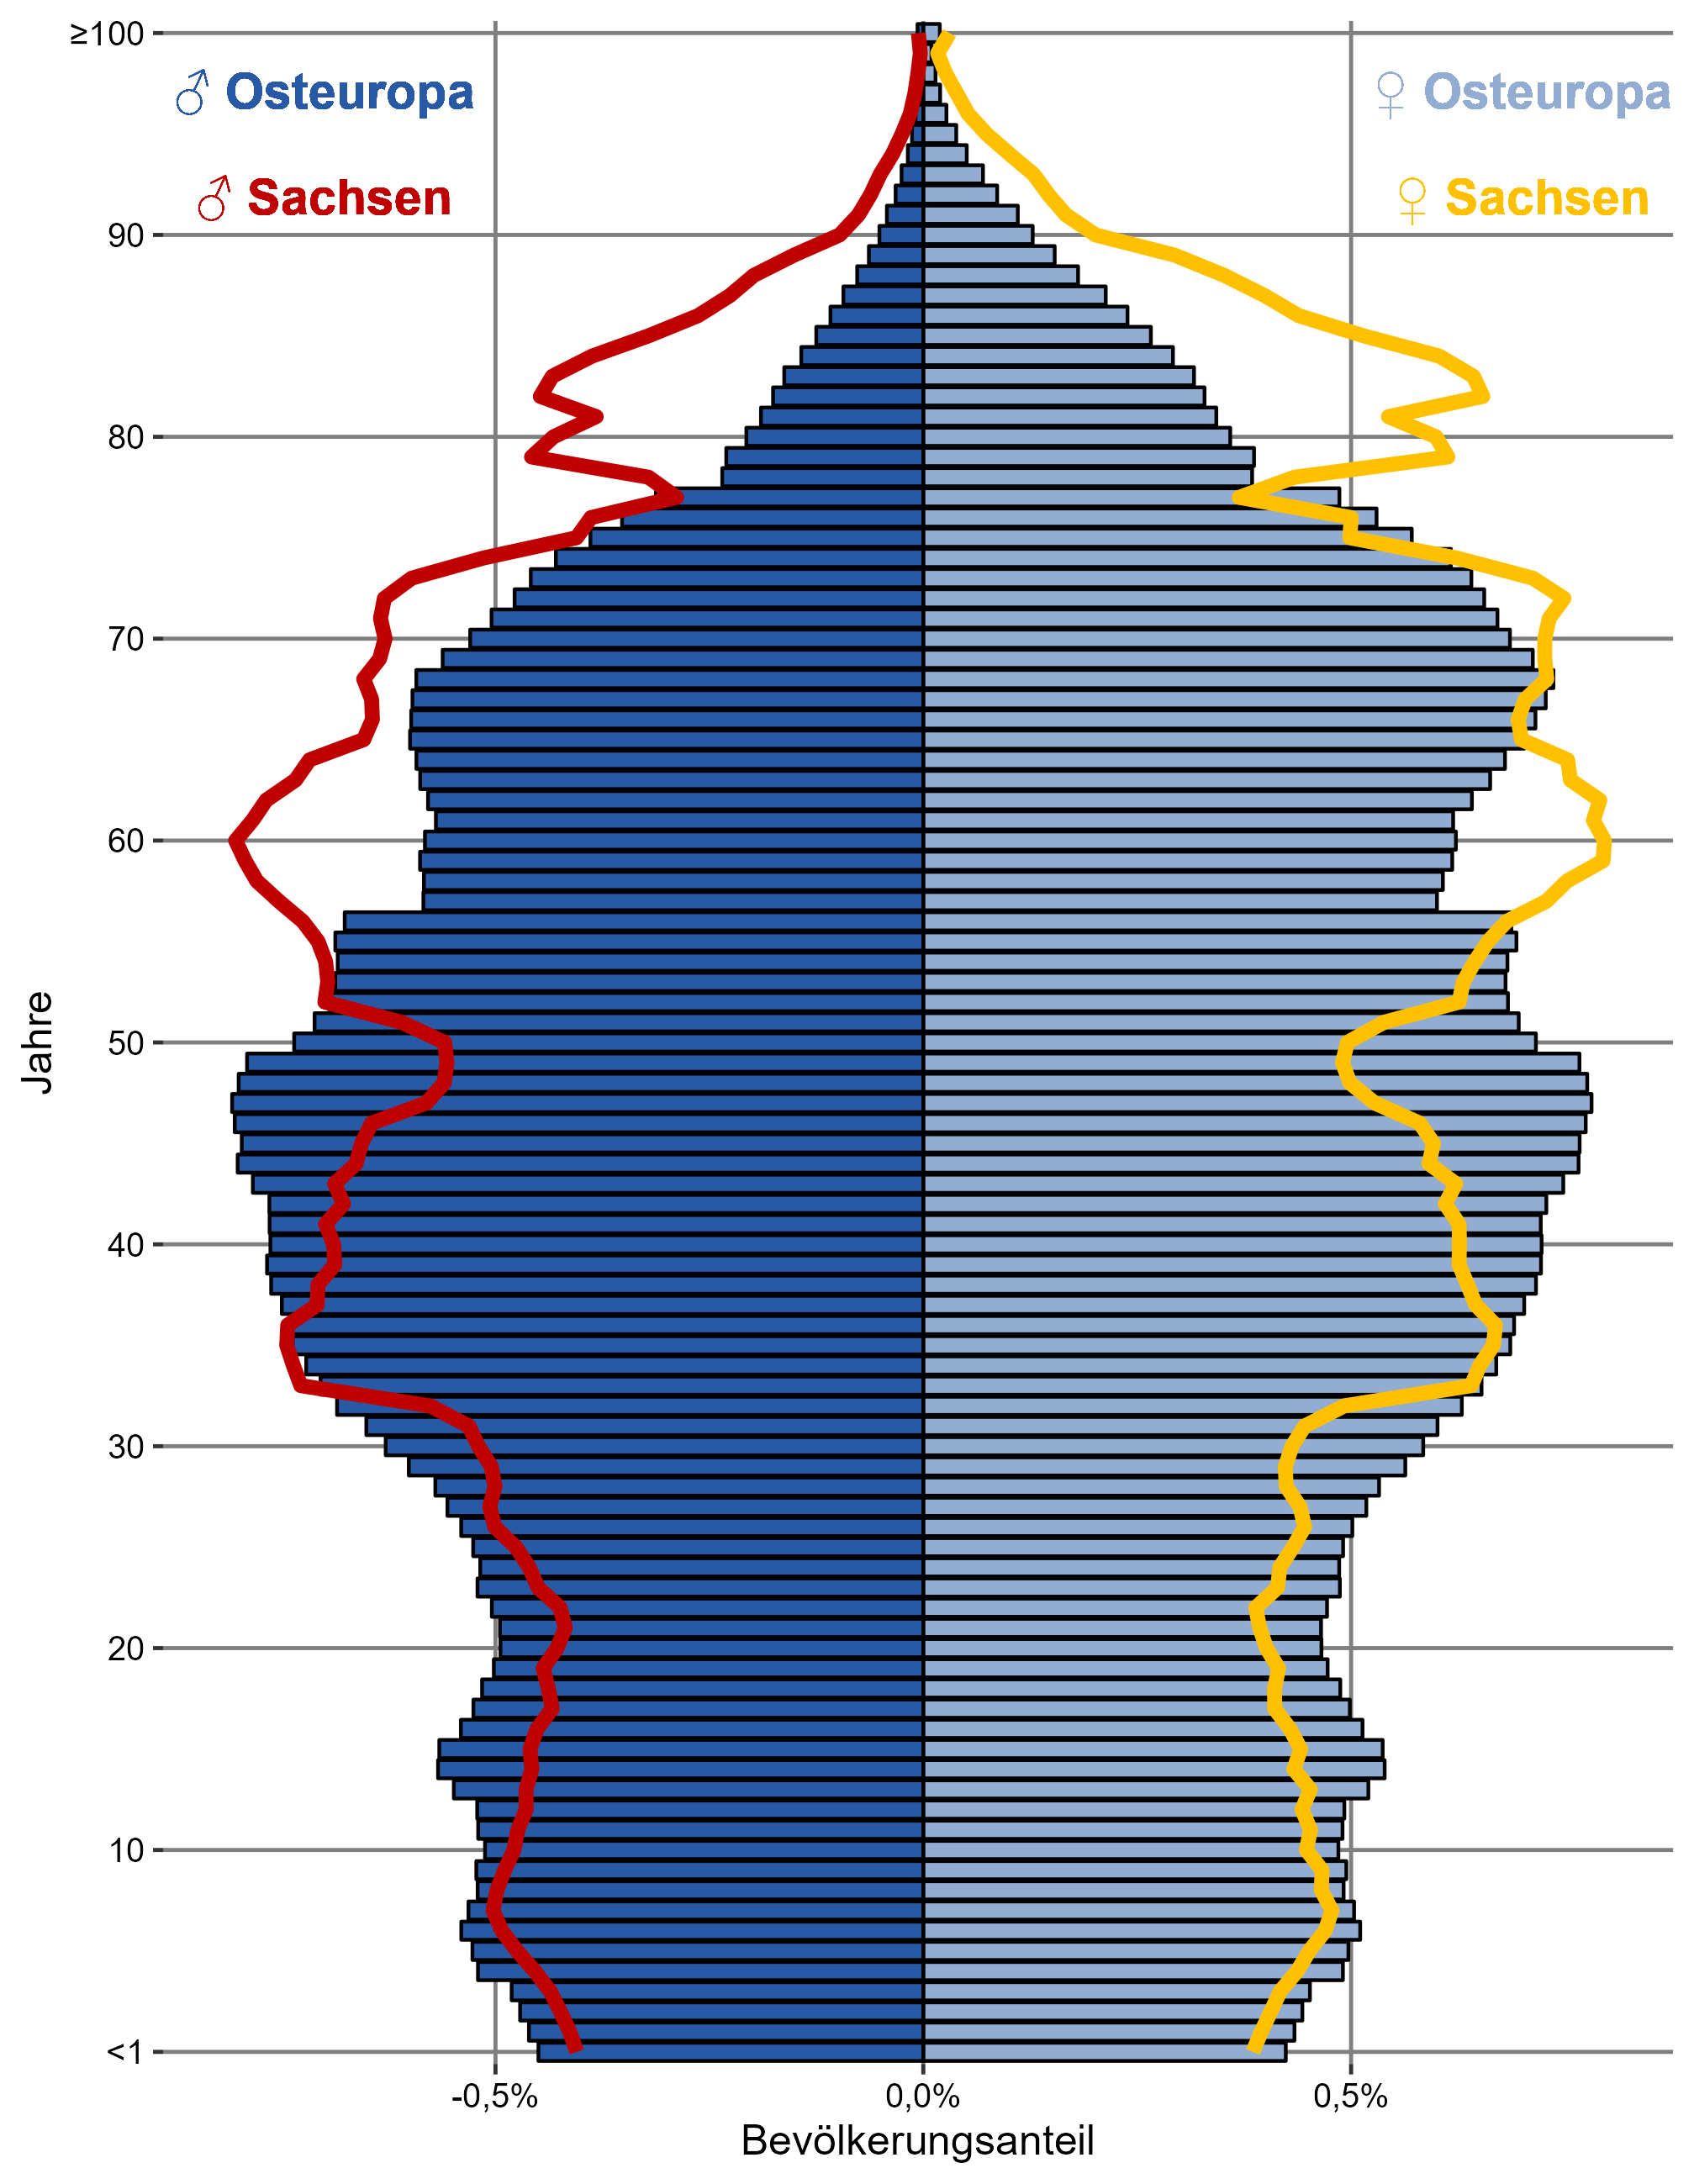
\includegraphics[width=\textwidth]{Bevoelkerungsverteilung}
	\begin{spacing}{1} \scriptsize
		Anm.: Bevölkerungsprognose für 2024; Baseline-Szenario; Stand 2021\\
		Quelle: Eurostat (2024); Ber. \& Dar. imreg (2024) \end{spacing}
\end{figure}

\begin{figure}[p]
	\addcontentsline{toc}{subsection}{Einwohnerzahl}
	{\centering \maps{Einwohnerzahl}}
	\label{map:einwohner}
	\karte{Einwohnerzahl}{2022}{Veränderung 2015 bis 2022}
	\begin{spacing}{1} \scriptsize
		Anm.: Stand 2022\\
		Quelle: Eurostat (2024); Ber. \& Dar. imreg (2024) \end{spacing}
\end{figure}


\begin{figure}[p]
	\addcontentsline{toc}{subsection}{Anzahl Haushalte}
	{\centering \maps{Anzahl Haushalte}}
	\label{map:haushalte}
	\karte{Haushalte}{2022}{Veränderung 2015 bis 2022}
	\begin{spacing}{1} \scriptsize
		Anm.: Stand 2022\\
		Quelle: Eurostat (2024); Ber. \& Dar. imreg (2024) \end{spacing}
\end{figure}


\begin{figure}[p]
	\addcontentsline{toc}{subsection}{Anzahl Haushalte in Städten}
	{\centering \maps{Anzahl Haushalte in Städten}}
	\label{map:haushaltestadt}
	\karte{Haushalte_Stadt}{2022}{Veränderung 2015 bis 2022}
	\begin{spacing}{1} \scriptsize
		Anm.: Stand 2022\\
		Quelle: Eurostat (2024); Ber. \& Dar. imreg (2024) \end{spacing}
\end{figure}


\begin{figure}[p]
	\addcontentsline{toc}{subsection}{Bevölkerungsdichte}
	{\centering \maps{Bevölkerungsdichte}}
	\label{map:bevdichte}
	\karte{Bevoelkerungsdichte}{2022}{Veränderung 2015 bis 2022}
	\begin{spacing}{1} \scriptsize
		Anm.: Stand 2022\\
		Quelle: Eurostat (2024); Ber. \& Dar. imreg (2024) \end{spacing}
\end{figure}


\begin{figure}[p]
	\addcontentsline{toc}{subsection}{Bevölkerungsveränderung}
	{\centering \maps{Bevölkerungsveränderung}}
	\label{map:bevrate}
	\karte{Bevoelkerungsveraenderung_Rate}{2021}{Veränderung 2015 bis 2021}
	\begin{spacing}{1} \scriptsize
		Anm.: Bevölkerungsveränderung je Tsd. Einwohner; Stand 2021\\
		Quelle: Eurostat (2024); Ber. \& Dar. imreg (2024) \end{spacing}
\end{figure}


\begin{figure}[p]
	\addcontentsline{toc}{subsection}{Natürliche Bevölkerungsveränderung}
	{\centering \maps{Natürliche Bevölkerungsveränderung}}
	\label{map:natbevrate}
	\karte{NatBevoelkerungsveraenderung_Rate}{2021}{Veränderung 2015 bis 2021}
	\begin{spacing}{1} \scriptsize
		Anm.: Bevölkerungsveränderung je Tsd. Einwohner; Natürliche Bevölkerungsveränderung = Lebendgeburten $-$ Sterbefälle; Stand 2021\\
		Quelle: Eurostat (2024); Ber. \& Dar. imreg (2024) \end{spacing}
\end{figure}


\begin{figure}[p]
	\addcontentsline{toc}{subsection}{Wanderungssaldo}
	{\centering \maps{Wanderungssaldo}}
	\label{map:wanderung}
	\karte{Wanderungssaldo_Rate}{$\varnothing$ Wanderungssaldo 2015 bis 2021}{Veränderung 2015 bis 2021}
	\begin{spacing}{1} \scriptsize
		Anm.: Wanderungssaldo je Tsd. Einwohner; Wanderungssaldo = Zuzüge $-$ Fortzüge; Stand 2021\\
		Quelle: Eurostat (2024); Ber. \& Dar. imreg (2024) \end{spacing}
\end{figure}


\begin{figure}[p]
	\addcontentsline{toc}{subsection}{Altersdurchschnitt (Median)}
	{\centering \maps{Altersdurchschnitt (Median)}}
	\label{map:alter}
	\karte{Medianalter}{2022}{Veränderung 2015 bis 2022}
	\begin{spacing}{1} \scriptsize
		Anm.: Stand 2022\\
		Quelle: Eurostat (2024); Ber. \& Dar. imreg (2024) \end{spacing}
\end{figure}


\begin{figure}[p]
	\addcontentsline{toc}{subsection}{Frauenquotient}
	{\centering \maps{Frauenquotient}}
	\label{map:frauen}
	\karte{Frauenquotient}{2022}{Veränderung 2015 bis 2022}
	\begin{spacing}{1} \scriptsize
		Anm.: Frauenquotient = $\frac{\text{Anzahl Frauen}}{\text{Anzahl Männer}} \times 100$; Stand 2022\\
		Quelle: Eurostat (2024); Ber. \& Dar. imreg (2024) \end{spacing}
\end{figure}


\begin{figure}[p]
	\addcontentsline{toc}{subsection}{Jugendquotient}
	{\centering \maps{Jugendquotient}}
	\label{map:jugend}
	\karte{Jugendquotient}{2022}{Veränderung 2015 bis 2022}
	\begin{spacing}{1} \scriptsize
		Anm.: Jugendquotient = $\frac{\text{Personen 0 - 14 Jahre}}{\text{Personen 15 - 64 Jahre}} \times 100$; Stand 2022\\
		Quelle: Eurostat (2024); Ber. \& Dar. imreg (2024) \end{spacing}
\end{figure}


\begin{figure}[p]
	\addcontentsline{toc}{subsection}{Altenquotient}
	{\centering \maps{Altenquotient}}
	\label{map:alte}
	\karte{Altenquotient}{2022}{Veränderung 2015 bis 2022}
	\begin{spacing}{1} \scriptsize
		Anm.: Altenquotient = $\frac{\text{Personen $\geq$ 65 Jahre}}{\text{Personen 15 - 64 Jahre}} \times 100$; Stand 2022\\
		Quelle: Eurostat (2024); Ber. \& Dar. imreg (2024) \end{spacing}
\end{figure}


\begin{figure}[p]
	\addcontentsline{toc}{subsection}{Altersabhängigkeitsquotient}
	{\centering \maps{Altersabhängigkeitsquotient}}
	\label{map:altersabh}
	\karte{Altersabhaengigkeitsquotient}{2022}{Veränderung 2015 bis 2022}
	\begin{spacing}{1} \scriptsize
		Anm.: Altersabhängigkeitsquotient = $\frac{\text{Personen 0 - 14 oder $\geq$ 65 Jahre}}{\text{Personen 15 - 64 Jahre}} \times 100$; Stand 2022\\
		Quelle: Eurostat (2024); Ber. \& Dar. imreg (2024) \end{spacing}
\end{figure}


\begin{figure}[p]
	\addcontentsline{toc}{subsection}{Bevölkerungsprognose 2050}
	{\centering \maps{Bevölkerungsprognose 2050}}
	\label{map:bevprog}
	\karte{Bevoelkerungsprognose}{2050}{Veränderung 2024 bis 2050}
	\begin{spacing}{1} \scriptsize
		Anm.: Basisvorausberechnung; Stand 2020\\
		Quelle: Eurostat (2024); Ber. \& Dar. imreg (2024) \end{spacing}
\end{figure}

